\begin{savequote}[75mm]
I've often said that my rats have taught me much more than I've taught them.
\qauthor{B. F. Skinner}
\end{savequote}

\chapter{Experiment description}
\label{chap:experiment}


\textcolor{red}{Aqui você precisa colocar um parágrafo explicando que os dados foram coletados no nosso laboratório e citar quem foi responsável pela coleta dos dados: Gabriela e Elyezyer. Caso contrário, dará a impressão de que foi você que os coletou. Coloque que foi um trabalho colaborativo com outros dois alunos um de mestrado, outro de doutorado, etc, etc. Explique o contexto para deixar bem separado o que é a sua contribuição.}

The present work is part of a bigger collaboration of our research group. The following experiments were carried out by a PhD student Gabriela Chiufa and a Master's student Eliezyer Fermino, and the present contribution builds analysis upon their collected data.

\section{The task}
    The subjects were 8 adult naive male Wistar rats (12 - 16 weeks old, weighing 380 - 400~g). The animals were housed individually in a 12h light/dark cycle with the light turned on at 7 am. They were food-deprived to gradually reach and then maintain 85\% of their free-feeding weight. Animals were handled according to the experimental protocol approved by UFABC's Ethics Committee (Comitê de Ética de Uso Animal CEUA-UFABC) \footnote{under the protocols 2905070317 (group 1) and 1352060217 (group 2)}. All procedures were conducted during the light cycle.
    
    Animals were trained in an operant chamber developed in our laboratory, totally controlled by an Arduino uno, and made of acrylic plastic. The box has a \textit{nosepoke}, which is a hole equipped with an infrared emitter-sensor that detects when the animal inserts its snout. In the same wall there is a drinker coupled to a lickometer, which is a nozzle that the animal licks to obtain water-sucrose solution. Before the nozzle there is a gate, controlled by an arduino board coupled to a stepper motor, that limits the animal access. 
    
    \begin{figure}
        \centering
        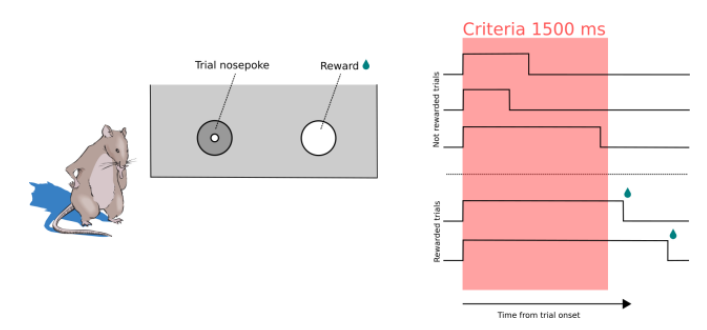
\includegraphics[width=\textwidth]{figures/tarefa_eli.png}
        \caption[Our DRRD task]{Our DRRD task. If the animal stays in the nosepoke for longer than the criteria, it can collect a reward. Taken with permission from \cite{Eliezyer2018}}
        \label{fig:task}
    \end{figure}

\section{Training schedule}
    First, the animals were trained to nose poke in a continuous schedule of reinforcement (CR), in which every nosepoke was rewarded independent of duration, by a reward of four licks of a 50\% glucose solution. To conclude this phase, the animal had to nose poke at least 100 times on a 60 minutes session. 
    
    After reaching the target number of nose pokes, animals were trained with a Differential Reinforcement of Response Duration (DRRD) procedure. The DRRD consisted on a similar task, with the difference that only long trials were rewarded. In order to receive the reward (licks of a water-sucrose solution), the animal had to poke the hole and hold it inside for a time equal or longer than the defined criterion of 1500ms. The trials were self initiated and self ended, and even when the animals didn't reach the time criteria, they were free to start a new trial. Animals had at most one training session per day, both in CR and in the subsequent DRRD. All sessions were video recorded. More details about the training schedule can be found in Reyes et al.~\cite{ReyesDRRD}.

    \subsection{Rationale}
        The central distinction of this version of the DRRD task is the speed of behavior acquisition. It was developed by our group to enable recording of neurons through learning in a single session, and most of the specificities of this task were defined with this aim.
        
        Some DRRD protocols define a time window for the reinforcement, i.e., only responses within a minimum and a maximum interval are reinforced. Thus if the animal responds (nosepoking, or pressing a lever) for too long, it receives no reward. Previous results from our group showed that the upper limit is not necessary for learning, at least at the beginning of the training. Hence, we removed this upper criterion. We believe this modification does not change the nature of the task -- it is still a timing task. We argue that the upper criterion is unnecessary because the incentive to get rewarded as soon as possible is sufficient to enforce a penalty for longer responses. Behavioral results indicate this is the case: animals' responses peak around the criterion, and very long responses are uncommon.